\chapter{TaCに関する資料}
\label{appTac}

%==============================================================================
\section{CPUの概要}
TaCで使用できるデータの形式,
CPU内部のレジスタ構成,
機械語命令について説明する.

\subsection{データ形式}
\figref{tacData}にTaCが扱うことができるデータ形式を示す.
16ビットの整数データと,16ビットのアドレスデータの他に,
8ビットのデータを扱うことができる.
16ビットのデータはCPUの内部でもメモリやI/Oでも使用できる.
メモリやI/Oの16ビットデータにアクセスする場合は偶数番地を用いる.
8ビットデータはメモリとI/Oの読み書きだけに使用できる.
メモリやI/Oの8ビットデータにアクセスする場合は,
CPUレジスタの下位8ビットが使用される.

\begin{myfig}{btp}{データ形式}{tacData}
  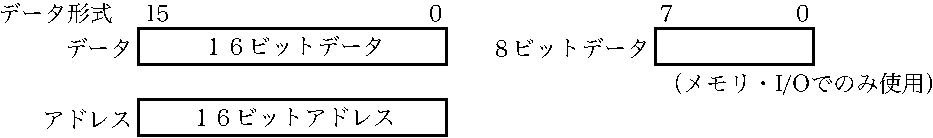
\includegraphics[scale=0.7]{Tbl/TaC7a-instruction-p1-1-crop.pdf}
\end{myfig}

\subsection{CPUレジスタとPSW}
\figref{tacRegPsw}にCPU内部のレジスタなどを示す.
レジスタはどれも16ビット幅である.
CPUレジスタは,
汎用のG0からG11,
フレームポインタとして使用するFP,
カーネルモード用のスタックポインタSSP,
ユーザモード用のスタックポインタUSPからなる.
これらは全て計算用にもアドレス用にも使用できる.
FP,SSP,USPは,以下に説明する特別な意味も持っている.

FPはフレームポインタ相対アドレッシングモードで使用できる.
このアドレッシングモードを用いると,
スタックフレーム内のローカル変数や関数引数へ,
1ワードの機械語命令でアクセスできる.

SSPはカーネルモードでSPの位置にマップされスタックポインタとして使用される.
USPはユーザモードでSPの位置にマップされスタックポインタとして使用される.
USPは最後のレジスタとして常時マップされており,
カーネルモードでもUSPをアクセスすることができる.

PSWはPCとFLAGからなる.
PCはプログラムカウンタのことである.
FLAGには,計算結果で変化するV,C,S,Zと,
割込み許可E,カーネルモードPの各ビットがある.
割込みが発生するとPCとFLAGが順にカーネルスタックにPUSHされた後で,
割込みが禁止されカーネルモードに切り換わる
(Eビットが0,Pビットが1になる).

\begin{myfig}{btp}{CPU内部の記憶装置}{tacRegPsw}
  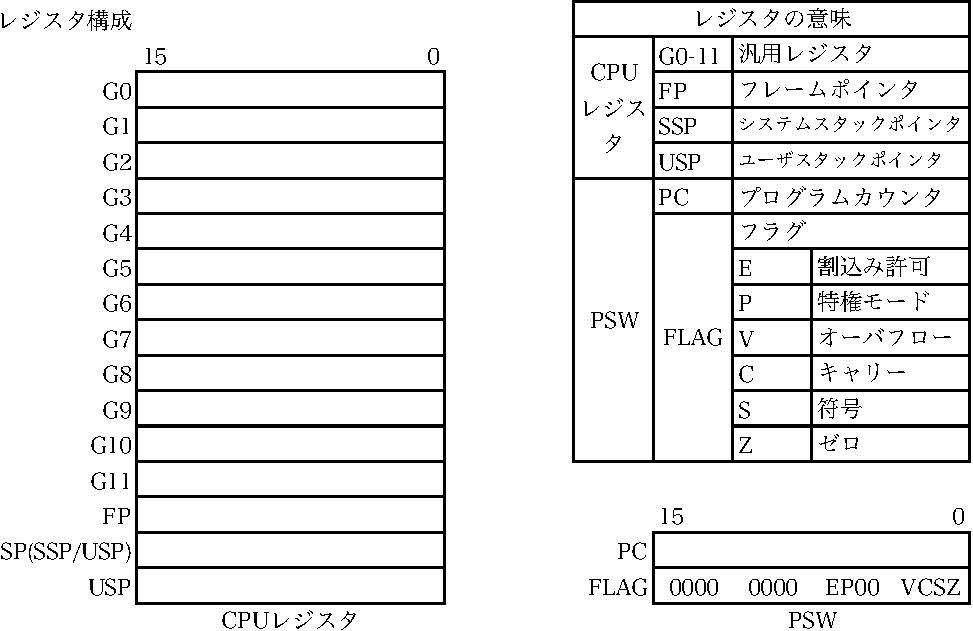
\includegraphics[scale=0.7]{Tbl/TaC7a-instruction-p1-3-crop.pdf}
\end{myfig}

\subsection{機械語命令}
\label{tacMachineIns}
\figref{tacInsTbl}にTaCの機械語命令の一覧表を示す.
IN,OUT,RETI,EI,DI,HALTは,
カーネルモードでしか使用できない\emph{特権命令}である.
SVC命令はシステムコールを発行するためにSVC割込みを発生する.

ほとんどの転送命令と計算命令で8種類のアドレッシング・モードが使用できる.
Direct,Indexed,Immediateの
三つのアドレッシング・モードを使用する場合は2ワードの機械語命令になる.
他のアドレッシング・モードの場合は全て1ワード命令である.

Byte Register Indirect アドレッシング・モードだけが,
メモリの8ビットデータをアクセスする.
Byte Register Indirect アドレッシング・モードの
ST命令は,CPUレジスタの下位8ビットをメモリに書き込む.
ST以外の命令は,メモリから読み出した8ビットデータの上位に
\|00h|を付加した16ビットデータに変換して使用する.

\begin{myfig}{btp}{命令表}{tacInsTbl}
  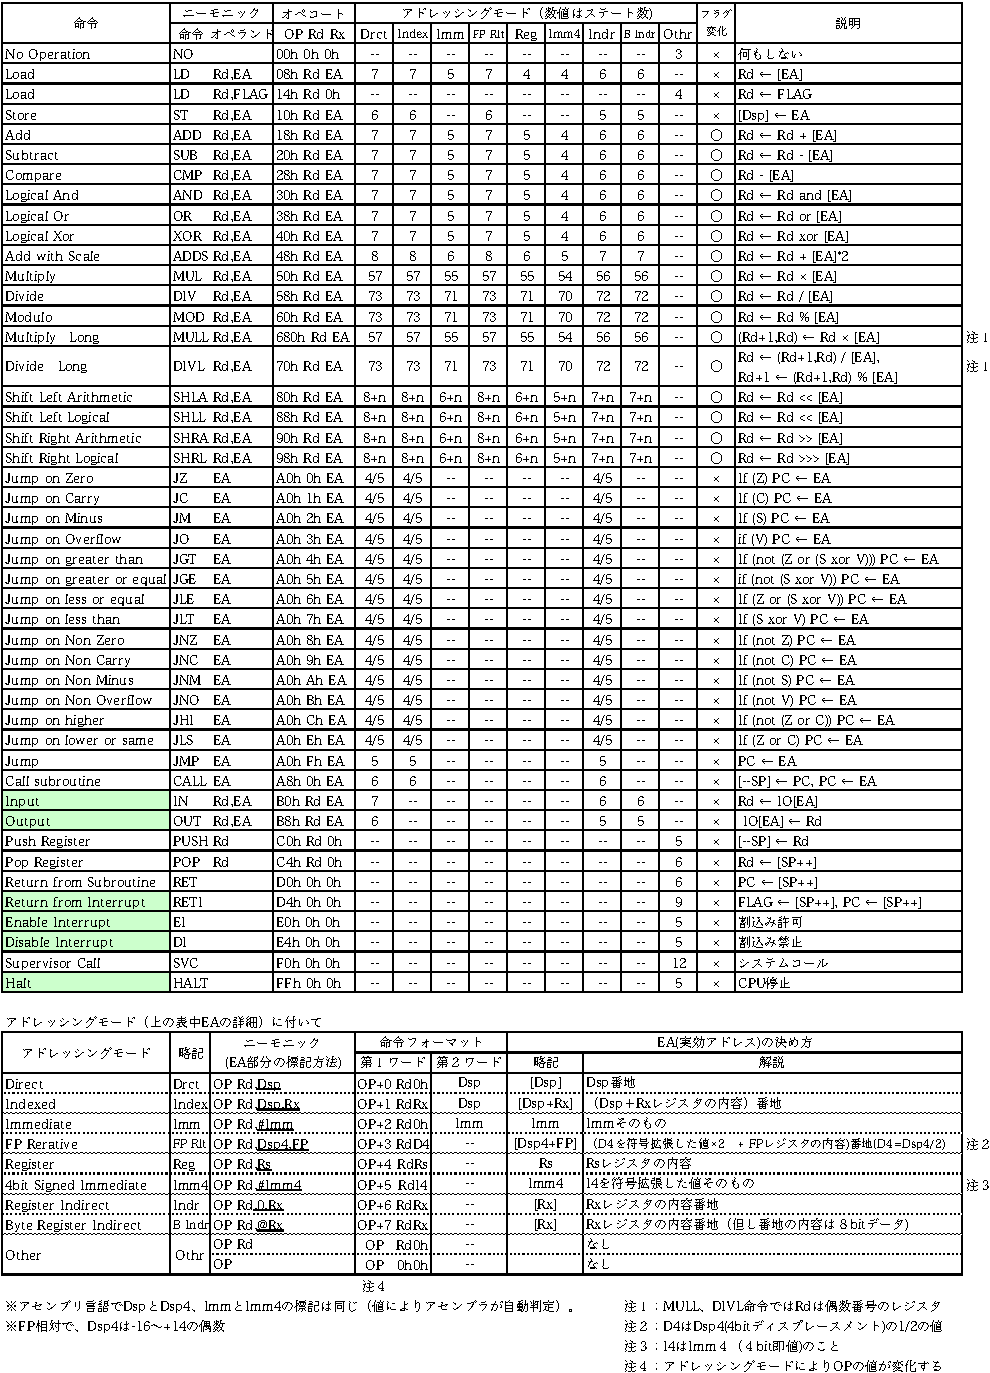
\includegraphics[scale=0.94]{Tbl/TaC7a-instruction-p2-crop.pdf}
\end{myfig}

%==============================================================================
\newpage
\section{メモリマップとI/Oマップ}
\figref{tacMap}にTaCのメモリマップとI/Oマップを示す.
メモリやI/Oは8ビット毎にアドレス付けされており,
8ビットデータ,16ビットデータのどちらも読み書きできる.
アドレッシング・モードによって,8ビットデータと16ビットデータの区別をする.
16ビットデータは偶数アドレスを指定してアクセスしなければならない.

\subsection{メモリ空間}
TaCのメモリ空間は\|0000h|から\|FFFFh|の64KiBである.
16ビットデータは偶数アドレスからの2バイトに配置され,
偶数アドレスを指定してアクセスする.
16ビットデータにアクセスするには,
Byte Register Indirect モード\emph{以外}のアドレッシング・モードを用いる.
8ビットデータにアクセスするには,
Byte Register Indirect モードを用いる.

メモリ空間の最初から56KiBは自由に使用できるメモリであり,
ここにTacOSのカーネルやユーザプロセスがロードされる.
\|E000h|から\|EFFFh|まではVRAMが配置されている.
VRAMにASCIIコードを書き込むと対応する文字がディスプレイに表示される.
VRAMのアドレスがディスプレイの表示位置に対応する.
\|F000h|から\|FFDFh|はIPL(ROM)が配置される.
IPLはマイクロSDカードからTacOSを読み出して起動する.
\|FFE0h|から\|FFFFh|は割込みベクタ領域である.
16種類の割込みに対応するハンドラの入口番地をTacOSがセットする.

\subsection{I/O空間}
TaCのI/O空間は\|00h|から\|FFh|の256Bである.
I/O空間のアドレス幅は8ビットだが,
IN,OUT命令ではI/Oアドレスが16ビットで表現される.
I/Oアドレスの上位8ビットは\|00h|になるようにする.
上位8ビットが\|00h|以外になった場合の動作は保証されない.

メモリ空間と同様に8ビットデータと16ビットデータの両方を読み書きできる.
8ビットデータと16ビットデータの区別は,
IN,OUT命令のアドレッシングモードにより行う.
I/Oの8ビットデータにアクセスするには,
Byte Register Indirect モードを用いる.

\begin{myfig}{btp}{メモリマップとI/Oマップ}{tacMap}
  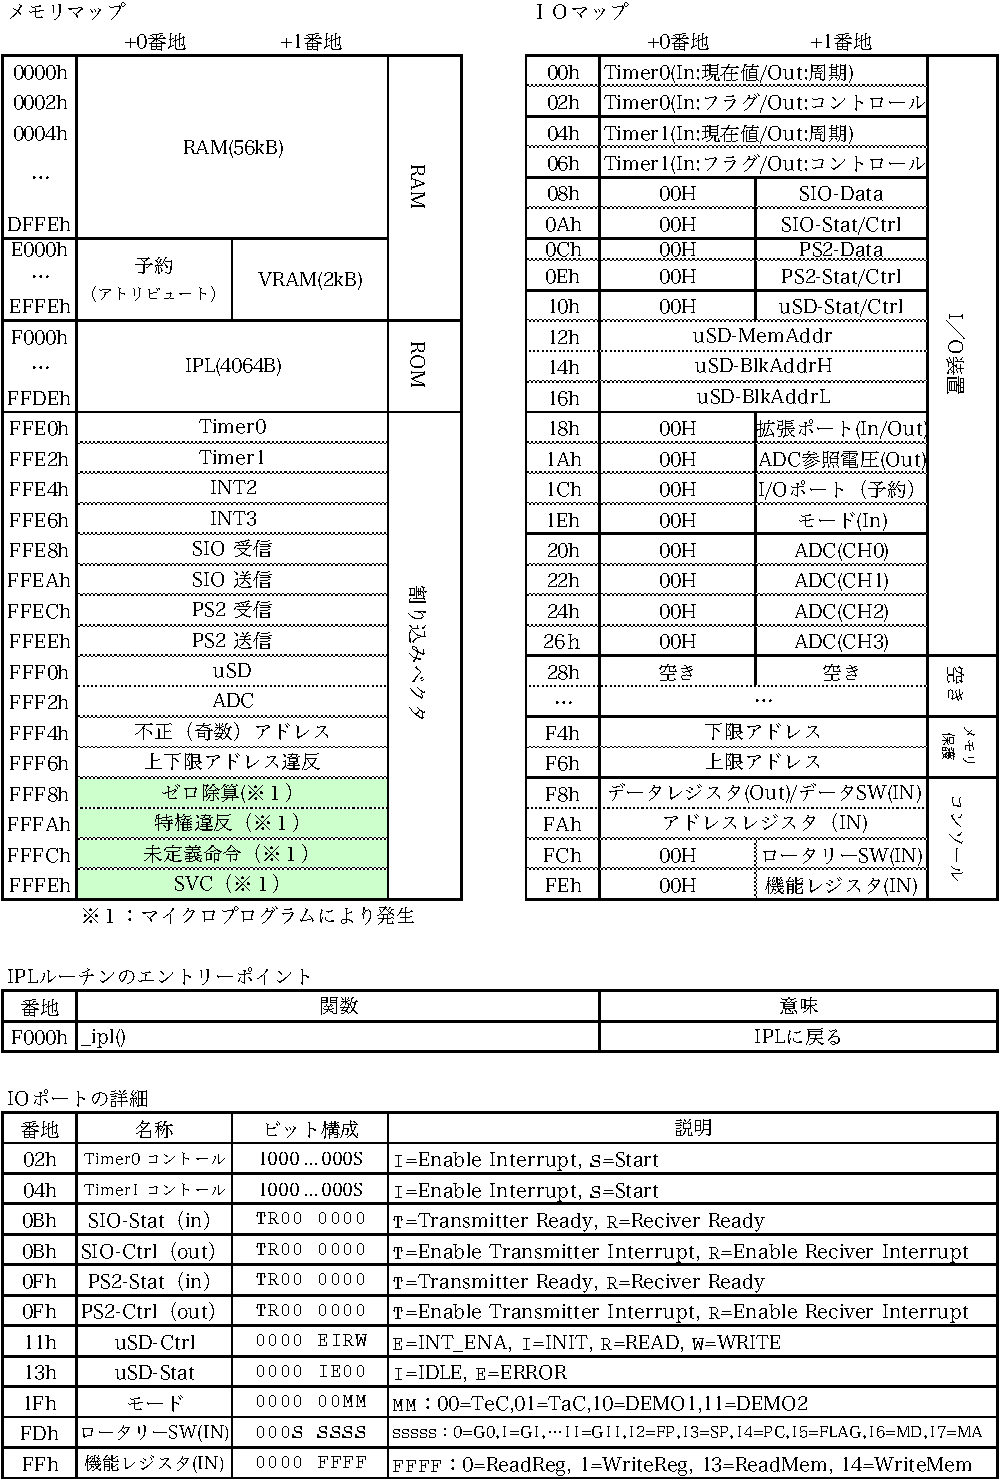
\includegraphics[scale=0.8]{Tbl/TaC7a-instruction-p4-crop.pdf}
\end{myfig}
